
\documentclass[12pt]{article}

\usepackage{scicite}
\usepackage{times}
\usepackage{graphicx}
\usepackage{hyperref}
\usepackage{enumitem}
\usepackage{amsmath}
\usepackage[utf8]{inputenc}
\usepackage{longtable}

\topmargin -1.5cm
\oddsidemargin 0.0cm
\textwidth 16cm 
\textheight 23.5cm
\footskip 1.0cm

\newenvironment{sciabstract}{%
\begin{quote} \bf}
{\end{quote}} 

\newcounter{lastnote}
\newenvironment{scilastnote}{%
  \setcounter{lastnote}{\value{enumiv}}%
  \addtocounter{lastnote}{+1}%
  \begin{list}%
  {\arabic{lastnote}.}
  {\setlength{\leftmargin}{.22in}}
  {\setlength{\labelsep}{.5em}}
}
{\end{list}}

\title{Assignment 3} 

\author
{Filipe Pires [85122], João Alegria [85048]\\
\\
Information Retrieval\\
\normalsize{Department of Electronics, Telecommunications and Informatics}\\
\normalsize{University of Aveiro}\\
} 

\date{\today{}}

%%%%%%%%%%%%%%%%% END OF PREAMBLE %%%%%%%%%%%%%%%%

\begin{document} 
\baselineskip18pt
\maketitle 

\section{Introduction}

This report was written for the discipline of 'Information Retrieval' and 
describes the implementation and evaluation of a ranked retrieval method that 
uses the indexes created with the solutions developed for the previous assignments.

We include the correction of design flaws of the delivery done prior to this one
and the updates applied both to the text corpus indexation and to our class diagram.
We also provide the instructions on how to run our code.

Along with the description of the solution, we also present the results of our
calculations to evaluate the solution and determine its efficiency according to 
the metrics proposed for this last assignment \cite{assign3}.
All code and documentation is present in our public GitHub project at 
\url{https://github.com/joao-alegria/RI}. 

\newpage
\section{Re-Indexing the Corpus}

In order to make query searches flexible, it was proposed to us the reindexation
of the text corpus considering not only the document titles but also their abstracts.
This turned out to be quite challenging due to its computational weight, as 
the abstracts were much larger than the titles.
The initial index occupied 500Mb in disk, whereas the reindexation was over 3Gb large.

There were 2 approaches when adding the abstract processing to our indexing process. 
The first one would consist in dealing with titles and abstracts separately,
creating independent index entries for both. 
This approach has the advantage of simplifying the process of verification of 
appearance of a given term in titles, abstracts or both, since they would be 
stored in different structures.
It has however the clear disadvantage of requiring far more disk space to store
all the information and introducing redundancy and unnecessary repetitions.

With this in mind, we went for another strategy, consisting of concatenating 
both fields and processing the resulting text as a whole.
This approach's advantage and disadvantage are inverted when compared to the 
previous, since the redundancy no longer exists but it becomes impossible to
distinguish the field a term appears at.
Our choice was based on the analysis of the requirements for the ranked retriever
we wanted to implement, as there seemed to be no need to keep the notion of where
each term appeared at in each document.
This also made the code adaptations to the indexing pipeline more straightforward 
and, as we previously mentioned, the final size in disk of the index smaller.
The execution time of this pipeline thankfully did not evolve as fast as the
disk space, passing from 20 minutes without the abstract to approximately 1 hour
and 20 minutes with it.

\begingroup
\addtolength\leftmargini{-0.4in}
\addtolength\baselineskip{-0.05in}
\begin{quote}
\begin{verbatim}
PMID- 10605436
(...)
TI  - Concerning the localization of steroids in centrioles
      and basal bodies by immunofluorescence.
PG  - 255-60
AB  - Specific steroid antibodies, by the immunofluorescence 
      technique, regularly reveal fluorescent centrioles and 
      cilia-bearing basal bodies in target and nontarget cells. 
      Although the precise identity of the immunoreactive 
      steroid substance has not yet been established, it seems 
      noteworthy that exogenous steroids can be vitally 
      concentrated by centrioles, perhaps by exchange with 
      steroids already present at this level. This unexpected 
      localization suggests that steroids may affect cell
      growth and differentiation in some way different from the 
      two-step receptor mechanism.
(...)
\end{verbatim}
\end{quote}
\endgroup
\vspace{-10pt}
Above is an example of the existing information on the text corpus about one document.

\newpage
\section{Ranked Retrieval of Relevant Documents}

With an entirely functional index creator and a folder of generated indexes from
the corpus of text documents, it was now time to develop a program capable of
interpreting queries and returning the index entries most relevant to them.
In this chapter we describe our implementation of a query results ranked retriever
- that we called \texttt{Searcher}.
We also explain how we prepared it for memory limitations and present the 
updates done to our class diagram.

\subsection{Document Ranked Scores}

The file \texttt{Searcher.py} contains an abstract class called \texttt{Searcher}
that serves as a template for the implementations of results retriever classes.
For our purposes, we developed \texttt{IndexSearcher}, a class that extends from
\texttt{Searcher} and is capable of selecting which index files are required to 
answer a given query, assigning scores to indexed documents and returning those 
considered most relevant to the query according to these scores.

The step of determining which index files will be needed is done by 
\textit{retrieveRequiredFiles()} and is basically a comparison of each query 
term with the name of each index file.
As index files are named after the first and last terms it contains (separated
by an underscore) and as the entire index is alphabetically ordered, the function
simply determines where each term will be present and returns those index files. 
It is needless to say that, in order for the retrieval process to not be compromised, 
the same tokenizer used on the \texttt{CreateIndex.py} must be used now.
A special case occurs when the necessary information is cached, i.e. when the 
results are already present in memory. 
This memory management will be detailed in section \ref{memory}.

Calculating each document's score regarding a query is not as easy to explain. 
The function \textit{calculateScores()} is the one responsible for obtaining the 
relevant document IDs and the respective score values. 
To calculate the scores, it's necessary to iterate over all the selected index 
files and identify the lines were the query tokens appear, so that we have access 
to the documents where that specific term occurred.
As an execution time and memory consumption reduction mechanism, we implemented 
a champion list strategy to decrease our search space, meaning that we only 
consider the first \texttt{S} documents (\texttt{S} can be defined by the user), 
which is made easy by the fact that previously with our indexing process we 
already order the posting list (list of documents were a term appeared) by the 
tf-idf weight.

We then estimate the relevant documents, assuming that having at least one term 
of the query is enough but also considering that not all documents have the same 
relevance to the user because a document that has all the query terms may be more 
relevant that others with fewer.

\begin{equation}
  \label{score}
  Score_{d} = \sum_{t=0}^{nT} W_{qt} * W_{dt}
\end{equation}

\begin{equation}
  \label{simple}
  W_{qt} = 1 + \log(tf) * idf => Simplifying => W_{qt} = 1 * idf
\end{equation}

Scores are calculated to allow the ordering of the documents considered potentially
relevant. This calculation is done following the formulas above, where \ref{score} 
shows that the score of a document is obtained by the sum of the multiplications 
of the query term weight by the weight of the term in the document. 
This formula, although not too complex, can be simplified, as shown in \ref{simple}. 
Since the execution time when retrieving information is crucial, the simpler and 
straightforward the process is, the best for the user. 
The simplification that we implemented consists of assuming that each term occurs 
only once in the query, which doesn't compromise the performance of the search 
since the terms are still considered and the number of times a term appears in 
the query should not significantly affect the relevance of a document. 
This allows our process to simply skip the step of calculating the query term 
weights as shown in \ref{simple}, which can translates to crucial processing time speedup.

Once the scores are found, \textit{sortAndWriteResults()} does what its name 
suggests: sorts the documents by score and writes to a results file the first 
\texttt{limit} documents, where \texttt{limit} is passed as argument.

\subsection{Relevance Feedback}\label{rocchio}

We knew \texttt{IndexSearcher} was a very limited solution, as it considers 
documents as relevant only for the presence of query terms in their titles 
and/or abstracts.
So the idea of attempting to expand queries was introduced through feeding back
to the Searcher information that would help it fine tune its results.

The aim of relevance feedback is to try to steer the search process behavior 
in a way that guides the results to more relevant document.
This is accomplished by transforming the query vectors (consisting in the weights 
of each query term in the query) into new vectors closer to the trully
relevant documents and further away from the remainder.
The way we implemented this form of attempt to improve results was through the
well known algorithm Rocchio algorithm.

Rocchio was developed using the Vector Space Model like many other relevance 
feedback approaches. 
Descending from the SMART Information Retrieval System, the algorithm assumes 
that most users have a general conception of which documents should be denoted 
as relevant or non-relevant. 
With this information in mind, an improvement over the classic score values 
calculation is proposed by the following the formula \cite{rocchio}:

\vspace{-10pt}
\begin{equation}
  \vec{q}_{m} = \alpha\vec{q}_{0} + \beta\frac{1}{|D_{r}|} \sum_{ \vec{d}_{j} \in D_{r}} \vec{d}_{j} - \gamma\frac{1}{|D_{nr}|} \sum_{ \vec{d}_{j} \in D_{nr}} \vec{d}_{j}
\end{equation}
 
Where $\vec{q}_{0}$ is the original query vector, i.e. the weights of each term 
in the query, that in our context is simplified to $1 \times idf$; 
$D_{r}$ is the list of known relevant documents;
$D_{nr}$ is the list of known non-relevant documents; 
finally $\alpha$, $\beta$ and $\gamma$ are parameters that can be altered by the 
user to improve the performance of the algorithm. 

Developing the formula we end up with the addition of three vectors: 
the original query, the sum of all relevant document vectors and the sum of all 
non-relevant vectors, which when applying the formula and summing all the values 
of the resulting vector we achieve the new score of the document.

Taking a closer look at what the algorithm attempts to do, in a first analysis 
it appears to do the same for all documents, which could translate in maintaining 
the relations between them, but it's from our understanding that although true, 
(referring to the vector space model that the algorithm is based on) what's 
really happening is that the algorithm is trying to shift the query closer to 
the relevant documents by the addition of its middle point 
($\frac{1}{|D_{r}|} \sum_{ \vec{d}_{j} \in D_{r}} \vec{d}_{j}$) and distance it 
from the non-relevant documents through the substation of its middle point 
($\frac{1}{|D_{nr}|} \sum_{ \vec{d}_{j} \in D_{nr}} \vec{d}_{j}$).
This algorithm had a considerable impact in our system, which will be further 
explained in sections \ref{results} and \ref{discussion}.

We decided to implement 2 distinct approaches of providing feedback.
The first was a simulation of the user feedback and the other was a pseudo feedback. 
To achieve the first strategy we executed the information retrieval normally, 
obtaining the best results our system could supply and compared the obtained 
top K results with the gold standard supplied to us for the assignment. 
From those, the results that checked with the gold standard were considered as 
relevant documents and the remaining as irrelevant; 
this information was partially processed and persisted in files to make its 
further usage easier. 
A similar process was made to the pseudo feedback, being this one quite simpler 
since it only considers the relevant documents and defines them by selecting the 
top K values returned.

A Python script was developed to perform all of this automatically.
As it served only as an auxiliary function, we didn't took in consideration the 
execution time nor the memory usage, since the values it produces should ideally, 
in a real world situation, be selected and verified in a more controlled and reliable way.

\subsection{Memory Management} \label{memory}

When developing \texttt{Searcher}, we decided to implement an intelligent memory
usage strategy to take advantage of the unused memory that the system has available. 
By storing the terms and the respective champions needed to answer the queries 
performed in the system and the number of times the term is used, we can manage 
which terms and documents are in memory and which ones should we maintain.

The workflow that we adopted consisted in: if the program has memory available, 
it will store the terms used to answer the query being processed and the 
respective champion lists; if it detects that the memory limit is close to be 
surpassed, the internal cache is cleaned, leaving only one forth of what was 
originally there (the most used terms until then). 
This ensures that the most relevant terms are probably in memory and consequently 
will decrease the execution time, due to less I/O operations. 
After cleaning the internal cache the process verifies that memory was freed and 
continues writing the terms used which may become the new most used terms.

Below we present the diagram of all developed classes, including those for index 
creation and those for index querying.

\begin{figure}[h!]
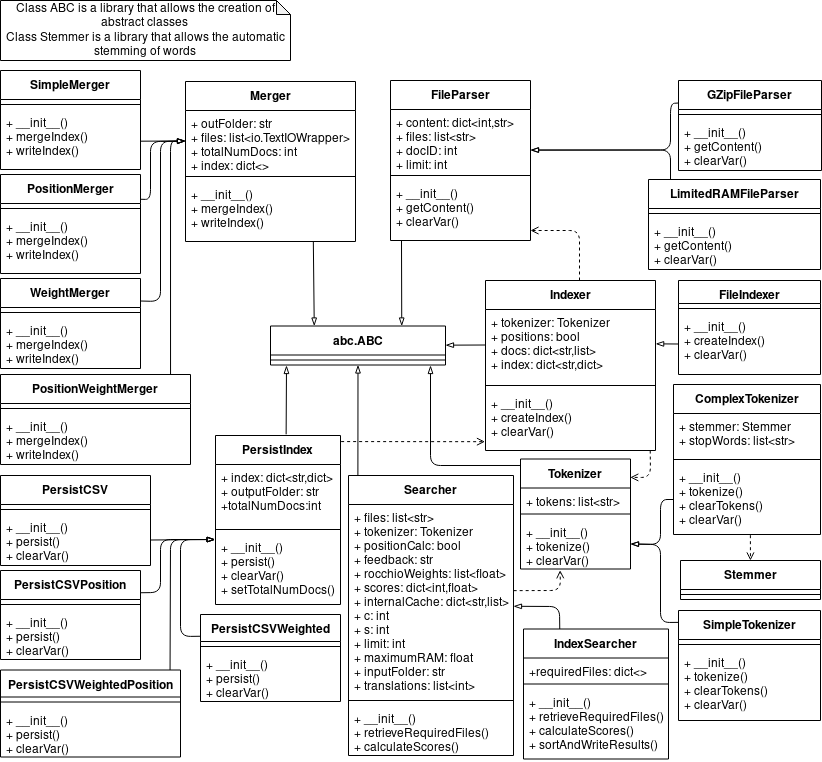
\includegraphics[width=\linewidth]{ClassDiagram_assign3.png}
\caption{Program's class diagram.}
\label{fig:classdiagram}
\end{figure}

\newpage
\section{Evaluation and Results Discussion}

In order to evaluate the quality of our solutions, with and without relevance 
feedback, we calculate an assortment of performance metrics.
The chosen metrics were: Precision, Recall, F-Measure, Mean Precision at rank 10, 
Mean Precision, Normalized Discounted Cumulative Gain, and all the averages in 
between the queries performed for all the previous metrics.
The implementation of the calculations was done in \texttt{QueryAnalyzer.py}.
Time related metrics were also considered, such as: Query Throughput and Median 
Query Latency, but for these we chose to use an auxiliary linux command line 
program called \texttt{time} which is able to summarize the system resources 
used in a program's execution.

In this chapter we explain the metrics used to evaluate the implemented ranked
retrieval, present the results of our evaluation and our discussion regarding 
them and attempt to understand what exactly are the solutions limitations.

\subsection{Evaluation Metrics} \label{metrics}

Precision and recall are one of the most used metrics in information retrieval.
The first is characterized by dividing the correct retrieved documents by the 
totality of retrieved documents. 
This metric provides the percentage of the retrieved documents that are really 
relevant for the user.
The second consists of dividing the correct retrieved documents by the totality 
of ideal correct documents. 
The result is the percentage of correct documents the system can present.

F-Measure (or F-Score) is a metric many times used to represent the system 
performance with only one value. 
This is accomplish by the combination of the two previous metrics, performing 
the harmonic mean between the two metrics through the following equation:

\begin{equation}
  Fs = \frac{2 \times P \times R}{P + R}
\end{equation}

Mean Precision is a variation of the Precision metric. 
Its formula is similar, the difference is that in this case the precision 
is calculated in the various ranks, i.e. it is calculated for every newly 
retrieved document and then the average of all the intermediate precisions 
is achieved, resulting in the mean of the precisions of the query result
(hence the name).
Mean Precision at rank 10 is described as the Mean Precision calculated just 
until rank 10 (unitl the $10^{th}$ value).

Normalized Discounted Cumulative Gain is a more complex metric that uses a graded 
relevance scale of documents to evaluate usefulness/gain of the returned results. 
The core idea with this metric is that relevant documents that are lower in the 
list should be penalized, since the important documents should be the first 
results provided. 
This is accomplished by the formula:

\begin{equation}
  DCG = \sum_{i=1}^{p} \frac{rel_{i}}{\log_{2}(i+1)}
\end{equation}

The normalization is then achieved by dividing this value by the ideal one, i.e.
having the relevances in order, the first documents considered the most relevant 
and so on.

Query Throughput is a time related metric that indicates how many queries can be 
processed in one second. 
It's obvious that it's ideal that the information gathering and ordering should 
take the least amount of time possible, so the higher the query throughput the better.

Finally, the Median Query Latency, as the name suggests, is the average time it
takes to process a query. 
Following the same logical line of thought of the previous metric, the lower 
this number is the better, since it means that more queries can be processed in 
less time.

\subsection{Results}\label{results}

The tests phase of the project was conducted with the help of \texttt{QueryIndex}
to execute the ranked retrievals and \texttt{QueryAnalyzer} to evaluate the results.
They considered the original dataset indexed with the updates mentioned in chapter 
1 and all 50 given queries.

\texttt{QueryIndex.py} works as the script that creates an instance of the 
\texttt{IndexSearcher} and, for each query, tells it to retrieve the best results.
The command works as follows:

\begingroup
\addtolength\leftmargini{-0.4in}
\addtolength\baselineskip{-0.05in}
\begin{quote}
\begin{verbatim}
$ python3 QueryIndex.py [-h] [-p] [-o outputFile] [-t tokenizer] 
  [-r limitRAM] [-f feedback] [-s rocchioScope] [-c numChamps] 
  [-l limit] queryFile indexFolder [a b g]
\end{verbatim}
\end{quote}
\endgroup

Here, \texttt{-h} is the option that presents the manual for the command usage.
Option \texttt{-p}, if present, tell the program that the index has the positions
of each term in each document along with the weights.
Option \texttt{-o} allows the definition of the output folder's name where the
results will be stored.
Option \texttt{-t} makes possible for the user to choose the type of tokenizer
to be used, and the alternatives are: 'simple' for the use of the 
\texttt{SimpleTokenizer} class, and 'complex' for the \texttt{ComplexTokenizer} class.
The chosen tokenizer must be the same used when indexing the text corpus.
Option \texttt{-r} allows the user to define the maximum amount of memory that can
be used by the process running the program.
Option \texttt{-f} makes possible for the user to choose a form of relevance 
feedback, so that there is a greater assurance that the returned documents are
actually relevant to the query.
The alternatives are: 'pseudo' and 'user'.
Options \texttt{-s}, \texttt{-c} and \texttt{-l} allow the definition of the 
number of retrieved documents considered for the Rocchio algorithm (applied in
the relevance feedback), the size of the champions list and the number of scores
to return (to store in the output files).
The previous arguments are all optional and the actual values for these arguments
must appear right after the respective options.
\texttt{QueryFile} and \texttt{indexFolder} are the only obligatory parameters,
as they tell the program where are the queries and the index files.
\texttt{A}, \texttt{b} and \texttt{g} are optional parameters that must be defined
if the relevance feedback is activated (if \texttt{-f} and \texttt{-s} are also
defined), as they correspond to the Rocchio algorithm's parameters $\alpha$,
$\beta$ and $\gamma$.

We executed \texttt{QueryIndex.py} for different combinations of parameters to
ensure its correct functioning and to search for the configuration with highest 
performances.
It was initially tested with indexes with positions and both types of tokenizers, 
although the remaining tests were all using only weights to reduce execution times
and only the complex tokenizer to remove noise and increase precision.
Then we tested the program with and without champions list (although this was
not done through the command's parameters) and for champions lists of different sizes.
Following we also varied the number of documents the program returned.
And finally we tested the program with relevance feedback, with both pseudo and
simulated user feedbacks, and with different Rocchio parameters values.

The presence of the champions list seemed to have no relevant impact on the 
overall performance, with tests at the time rounding 19\% of precision
(with a champions list of size $10^4$).
This feature was important for the execution times, as it reduced the search 
space of the program for each query without loosing valuable information.
What we later understood was that, if its size was reduced, the lost of useful
information and relevant documents started to have a big impact on the performance,
as for a list of size $10^3$ the precision dropped to about 16\%.

With the champions list at size $10^4$, we tried to reduce the number of results
returned from 100 to 50, 20 and 10. 
The later reached a precision of 26\%, which was good news to us.

Although pseudo feedback was also part of our tests, we knew \textit{a priori} 
that this would not influence the results at all, since it assumed that the first
results the program already considered more relevant were in fact relevant and 
increased their final scores.
User feedback, on the other hand, proved to have great value when tested.
To test this form of feedback, we varied the parameters \texttt{n} (number of 
retrieved documents considered for the Rocchio algorithm) between 5, 10 and 20
with the \texttt{a}, \texttt{b} and \texttt{g} parameters fixed at 1.0, 0.5 and
0.25 respectively.
The final precision for each \texttt{n} was: 28\%, 29\% and 29\%. 
At last we inverted the parameters variation in order to study the effects of 
$\alpha$, $\beta$ and $\gamma$.
To do this, we fixed \texttt{n} at 10 and tested the 3 parameters for values
between 0 and 1.
The values with the best precision were \texttt{$\alpha$ = 1.0}, 
\texttt{$\beta$ = 1.0} and \texttt{$\gamma$ = 0.1}, with a final precision of 31\%.
Table \ref{tab:tab1} (located at the end of this document) presents the queries results
and statistics of the best performance achieved for further analysis.
Other tables are present in our repository for different number of results returned 
and without relevance feedback.

\subsection{Discussion}\label{discussion}

So the tests results were presented in the previous section, and the seemingly
best combination of parameters was achieved with the available resources and 
developed features.
However, we did not content with accepting the facts and looked for logical
explanations to the influence of each factor on the final performance.
Here we share our thoughts on each observation made and attempt to explain why
the final performance is as it is.

The reason why champions lists reduce execution times has already been slightly 
discussed. 
This is mainly due to the fact that, before executing any computation on the index,
a resize of the search space is done to discard irrelevant documents;
It makes sense then that, if a sufficient amount of unnecessary computations are 
avoided, the query answering is significantly reduced.
This is also why champion lists too small have a negative impact on the overall 
performance, since there is a higher probability of discarding entries that in 
reality would be benefitial.

The fact that the number of results returned directly influences the results 
precision is also simple to understand.
As the performance metrics are applied to the returned documents and compared 
against a set of documents previously defined as relevant, it is necessary to 
understand in the first place that the gold standard provided was obtained and 
validated by humans. 
Although this standard brings into reality the largest limitations we face, further 
detailed in section \ref{limitations}, our system is still able of finding relevant 
documents and placing them at a higher rank. 
When increasing the size of the returned list, it increases the probability of 
including documents that our system considers relevant but may not actually be 
relevant at all.

The way the user feedback through the Rocchio algorithm works is: scores from 
documents considered not relevant to a given query by users must be lowered and 
scores from relevant documents must be increased.
Well, it is only natural that, when applied with appropriate scores regulation,
this feedback will positively influence the program's precision because it gives
"inside information" on what the user making the query is probably looking for.
And the more documents considered on the algorithm, the more the results will 
be closer to the truly relevant documents and further from the non relevant, as 
more documents from the results are affected by this regulatory feature.
The best parameter combination found for the algorithm was $\alpha=1, \beta=1 and \gamma=0.1$. 
This makes sense since what those values try to convey is that the original query 
results must be really relevant, that the values from the relevant document 
feedback are as relevant as the query (which is logical since it knows 
\textit{a priori} that those documents are truly relevant), and that the irrelevant 
results need to be considered but their importance is much smaller.
Referring to section \ref{rocchio}, one can understand that those values are 
reasonable based on the Vector Space Model, where the intention is to allow the 
shift of the query vector closer to relevant documents with $\beta=1$ and distance 
them from the irrelevant documents but not so much as to distance them again 
from the relevant ones, hence the $\gamma=0.1$.

In our analysis we only mention precision as a means of determining whether 
the variation of parameters was good or bad, but in reality our observations 
are also verified by the other metrics, only their evolution is not as 
straightforward to explain as precision's.
Nevertheless, we reached a few conclusions regarding other performance metrics
worth mentioning.

A low recall is common amongst all tests and, at first sight, it seems a bad sign.
However, it is actually expected to be low, since in many cases the amount of 
returned documents is usually very low compared to the entire list of documents 
from the index.

Another curious conclusion taken from our tests was the values obtained by the 
Normalized Discounted Cumulative Gain which as already explained in section 
\ref{metrics}, in summary represents how well the ordering of our results were 
presented, being the most relevant documents ideally present higher in the 
document list. 
Although not perfect, it was quite interesting to see that our ordering was 
acceptable, which we didn't expect from the poor precision values obtained.

\subsection{Implementation Limitations} \label{limitations}

So far we have explored ways of improving the program's performance through
limited, although relevant, strategies.
But the hard truth is that a precision of 30\% on a sort of search engine is not
exactly something to be very much proud of, or, at least, not the ideal value 
a regular user expects from such system.
In this section we attempt to understand why our solution is so limited and 
what could be done to greatly increase its quality.

Two major factors limit retrieval speed.
Index file size is directly correlated with this, as it will determine how long
will it take to find the query terms on the indexes. 
If we made them smaller, retrievals would be faster.
However, we kept their sizes as they were as we considered them more realistic 
than reducing them to small amounts of Mb.
The amount of memory available also naturally influences execution time.
We found that, without memory restrictions, the minimum amount of memory required 
for retrievals to work reasonably well is only 500Mb, taking in consideration 
that the index process was made with 2Gb of memory space.
Adding restrictions slows down retrieval but makes the program capable of managing
the used memory to lower values.
The final version responds to all 50 queries within 35 seconds, or 50 seconds 
if memory is restricted to 300Mb.
This means that in general the system is capable of accomplishing a query throughput
of 1.43 queries per second and a query latency of 0.7.

There are some facts that explain why a high precision is never achieved.
The first is the lack of consideration for synonym terms and similar and related 
words when retrieving the documents.
As the solution only searches for the exact terms on the query, there are many
occurrences of ignored documents that were in fact very much relevant but did not
use the exact same terminology.
One simple example we manually detected was with the word 'cancer' that in many 
of the truly relevant documents appeared only as 'carcinoma'.
This could be dealt with by introducing a new form of query expansion Thesaurus-based,
i.e. expanding the query terms by, for each term, adding synonyms and related words
present in a thesaurus of quick access.
There is, however, a high cost of manually producing a thesaurus and periodically 
updating it.

Another way of improving performance would be through query refinements based on
log mining.
What this means, in a very simplified manner, is to consider previously made
queries and the results that users chose the most to refine the new query retrievals
in a smart, automatic and adaptive way.
This is only achievable if a lot of data to analyse is available, and is a technique
very much explored by large search engines.

\section{Conclusions}

After completing the assignment, we drew a few conclusions regarding our
solutions and the whole concept of efficient indexing and information retrieval.

The biggest challenge we faced was definitely the implementation of the Rocchio 
algorithm.
Understanding it required the capacity to visually place the query vectors in a 
multidimensional space and interpret what the algorithm did and how could it be 
achieved programmatically.

Another big challenge was the memory management.
As there was a need to ensure a minimum amount of available memory for the internal
variables to be properly used and we wished to keep information from query to query,
this process was not trivial and required a lot of brainstorming and code changes 
to achieve its final version.
One limitation we were not able to surpass was that, when reading a line from an 
index file, although the content might only be partially stored in memory, the act
of reading is anatomic and so if the line is large enough it might surpass the 
defined memory restrictions.
This issue is intrinsic to the programming language chosen and we did not find a 
way to only partially read a line.

From this assignment, we take a deeper understanding of the way search engines 
and other information retrieval systems decide which elements can be considered
more relevant and appropriate to return.
Our research and development made us gain knowledge on powerful optimization 
techniques in a practical way and challenged us to use what we had previously
developed for the first assignments the best possible way.

The overall perspective of our performance regarding the project is very positive,
as we were able to make a detailed study on what was at our reach to achieve the 
most optimized solution we were able to.
We were also happy to discover that, when the problem of synonyms and related 
words was not very much present, the solution was able to achieve very high 
precisions within less than a second per query.
In terms of code structure, modularity and documentation, we were also very 
careful and find that the delivered code is properly presented to any developer.

\begin{thebibliography}{9}
  \bibliographystyle{Science}

  \bibitem{assign3}
    S. Matos,
    \textit{IR: Assignment 3},
    University of Aveiro,
    2019/20.

  \bibitem{rocchio}
    \textit{The Rocchio (1971) Algorithm},
    \url{https://nlp.stanford.edu/IR-book/html/htmledition/the-rocchio71-algorithm-1.html}
    Stanford University,
    2008,
    accessed in 12/2019.
  
\end{thebibliography}

\clearpage

\appendix
\section*{Appendix}

% Please add the following required packages to your document preamble:
% \usepackage{longtable}
% Note: It may be necessary to compile the document several times to get a multi-page table to line up properly
\begin{longtable}[c]{|l|l|l|l|l|l|l|}
  \hline
  Query & Precision & Recall & F1 & MeanPrecision & MeanPrecision@10 & NDCG \\ \hline
  \endhead
  %
  1 & 0.50 & 0.06 & 0.11 & 0.80 & 0.80 & 1.00 \\ \hline
  2 & 0.60 & 0.06 & 0.11 & 0.68 & 0.68 & 0.83 \\ \hline
  3 & 0.00 & 0.00 & 0.00 & 0.00 & 0.00 & 0.00 \\ \hline
  4 & 0.00 & 0.00 & 0.00 & 0.00 & 0.00 & 0.00 \\ \hline
  5 & 0.10 & 0.04 & 0.06 & 0.00 & 0.00 & 0.50 \\ \hline
  6 & 1.00 & 0.11 & 0.19 & 0.90 & 0.90 & 1.00 \\ \hline
  7 & 0.80 & 0.07 & 0.13 & 0.80 & 0.80 & 0.86 \\ \hline
  8 & 0.00 & 0.00 & 0.00 & 0.00 & 0.00 & 0.00 \\ \hline
  9 & 0.70 & 0.06 & 0.11 & 0.47 & 0.47 & 0.64 \\ \hline
  10 & 1.00 & 0.75 & 0.86 & 0.67 & 0.67 & 1.00 \\ \hline
  11 & 0.00 & 0.00 & 0.00 & 0.00 & 0.00 & 0.00 \\ \hline
  12 & 0.30 & 0.01 & 0.02 & 0.67 & 0.67 & 1.00 \\ \hline
  13 & 0.10 & 0.04 & 0.06 & 0.00 & 0.00 & 0.32 \\ \hline
  14 & 0.00 & 0.00 & 0.00 & 0.00 & 0.00 & 0.00 \\ \hline
  15 & 0.00 & 0.00 & 0.00 & 0.00 & 0.00 & 0.00 \\ \hline
  16 & 0.70 & 0.05 & 0.09 & 0.52 & 0.52 & 0.80 \\ \hline
  17 & 0.00 & 0.00 & 0.00 & 0.00 & 0.00 & 0.00 \\ \hline
  18 & 1.00 & 1.00 & 1.00 & 0.00 & 0.00 & 1.00 \\ \hline
  19 & 0.00 & 0.00 & 0.00 & 0.00 & 0.00 & 0.00 \\ \hline
  20 & 0.30 & 0.03 & 0.05 & 0.15 & 0.15 & 0.56 \\ \hline
  21 & 0.50 & 0.06 & 0.11 & 0.71 & 0.71 & 0.86 \\ \hline
  22 & 0.00 & 0.00 & 0.00 & 0.00 & 0.00 & 0.00 \\ \hline
  23 & 0.20 & 0.01 & 0.02 & 0.13 & 0.13 & 0.81 \\ \hline
  24 & 1.00 & 0.38 & 0.56 & 0.90 & 0.90 & 0.84 \\ \hline
  25 & 0.10 & 0.03 & 0.05 & 0.00 & 0.00 & 0.39 \\ \hline
  26 & 0.80 & 0.17 & 0.28 & 0.63 & 0.63 & 0.85 \\ \hline
  27 & 0.10 & 0.03 & 0.05 & 0.00 & 0.00 & 1.00 \\ \hline
  28 & 0.20 & 0.15 & 0.17 & 0.25 & 0.25 & 0.75 \\ \hline
  29 & 0.10 & 0.02 & 0.04 & 0.00 & 0.00 & 0.43 \\ \hline
  30 & 0.10 & 0.01 & 0.01 & 0.00 & 0.00 & 0.30 \\ \hline
  31 & 0.00 & 0.00 & 0.00 & 0.00 & 0.00 & 0.00 \\ \hline
  32 & 0.00 & 0.00 & 0.00 & 0.00 & 0.00 & 0.00 \\ \hline
  33 & 0.00 & 0.00 & 0.00 & 0.00 & 0.00 & 0.00 \\ \hline
  34 & 0.00 & 0.00 & 0.00 & 0.00 & 0.00 & 0.00 \\ \hline
  35 & 0.40 & 0.01 & 0.03 & 0.38 & 0.38 & 0.77 \\ \hline
  36 & 0.80 & 0.03 & 0.06 & 0.58 & 0.58 & 0.82 \\ \hline
  37 & 0.00 & 0.00 & 0.00 & 0.00 & 0.00 & 0.00 \\ \hline
  38 & 0.00 & 0.00 & 0.00 & 0.00 & 0.00 & 0.00 \\ \hline
  39 & 0.00 & 0.00 & 0.00 & 0.00 & 0.00 & 0.00 \\ \hline
  40 & 0.20 & 0.01 & 0.01 & 0.17 & 0.17 & 0.83 \\ \hline
  41 & 1.00 & 0.02 & 0.03 & 0.90 & 0.90 & 0.89 \\ \hline
  42 & 0.40 & 0.01 & 0.01 & 0.24 & 0.24 & 0.67 \\ \hline
  43 & 0.10 & 0.01 & 0.01 & 0.00 & 0.00 & 1.00 \\ \hline
  44 & 0.40 & 0.01 & 0.01 & 0.24 & 0.24 & 0.48 \\ \hline
  45 & 0.10 & 0.01 & 0.01 & 0.00 & 0.00 & 1.00 \\ \hline
  46 & 1.00 & 0.05 & 0.10 & 0.90 & 0.90 & 1.00 \\ \hline
  47 & 0.00 & 0.00 & 0.00 & 0.00 & 0.00 & 0.00 \\ \hline
  48 & 0.60 & 0.04 & 0.07 & 0.44 & 0.44 & 0.75 \\ \hline
  49 & 0.40 & 0.05 & 0.10 & 0.43 & 0.43 & 0.73 \\ \hline
  50 & 0.00 & 0.00 & 0.00 & 0.00 & 0.00 & 0.00 \\ \hline
  Avg & 0.31 & 0.07 & 0.09 & 0.25 & 0.25 & 0.49 \\ \hline
  \caption{Values for 10 documents, user feedback(1,1,0.1)}
  \label{tab:tab1} 
  \end{longtable}


\end{document}




















